\begin{figure}
\centering
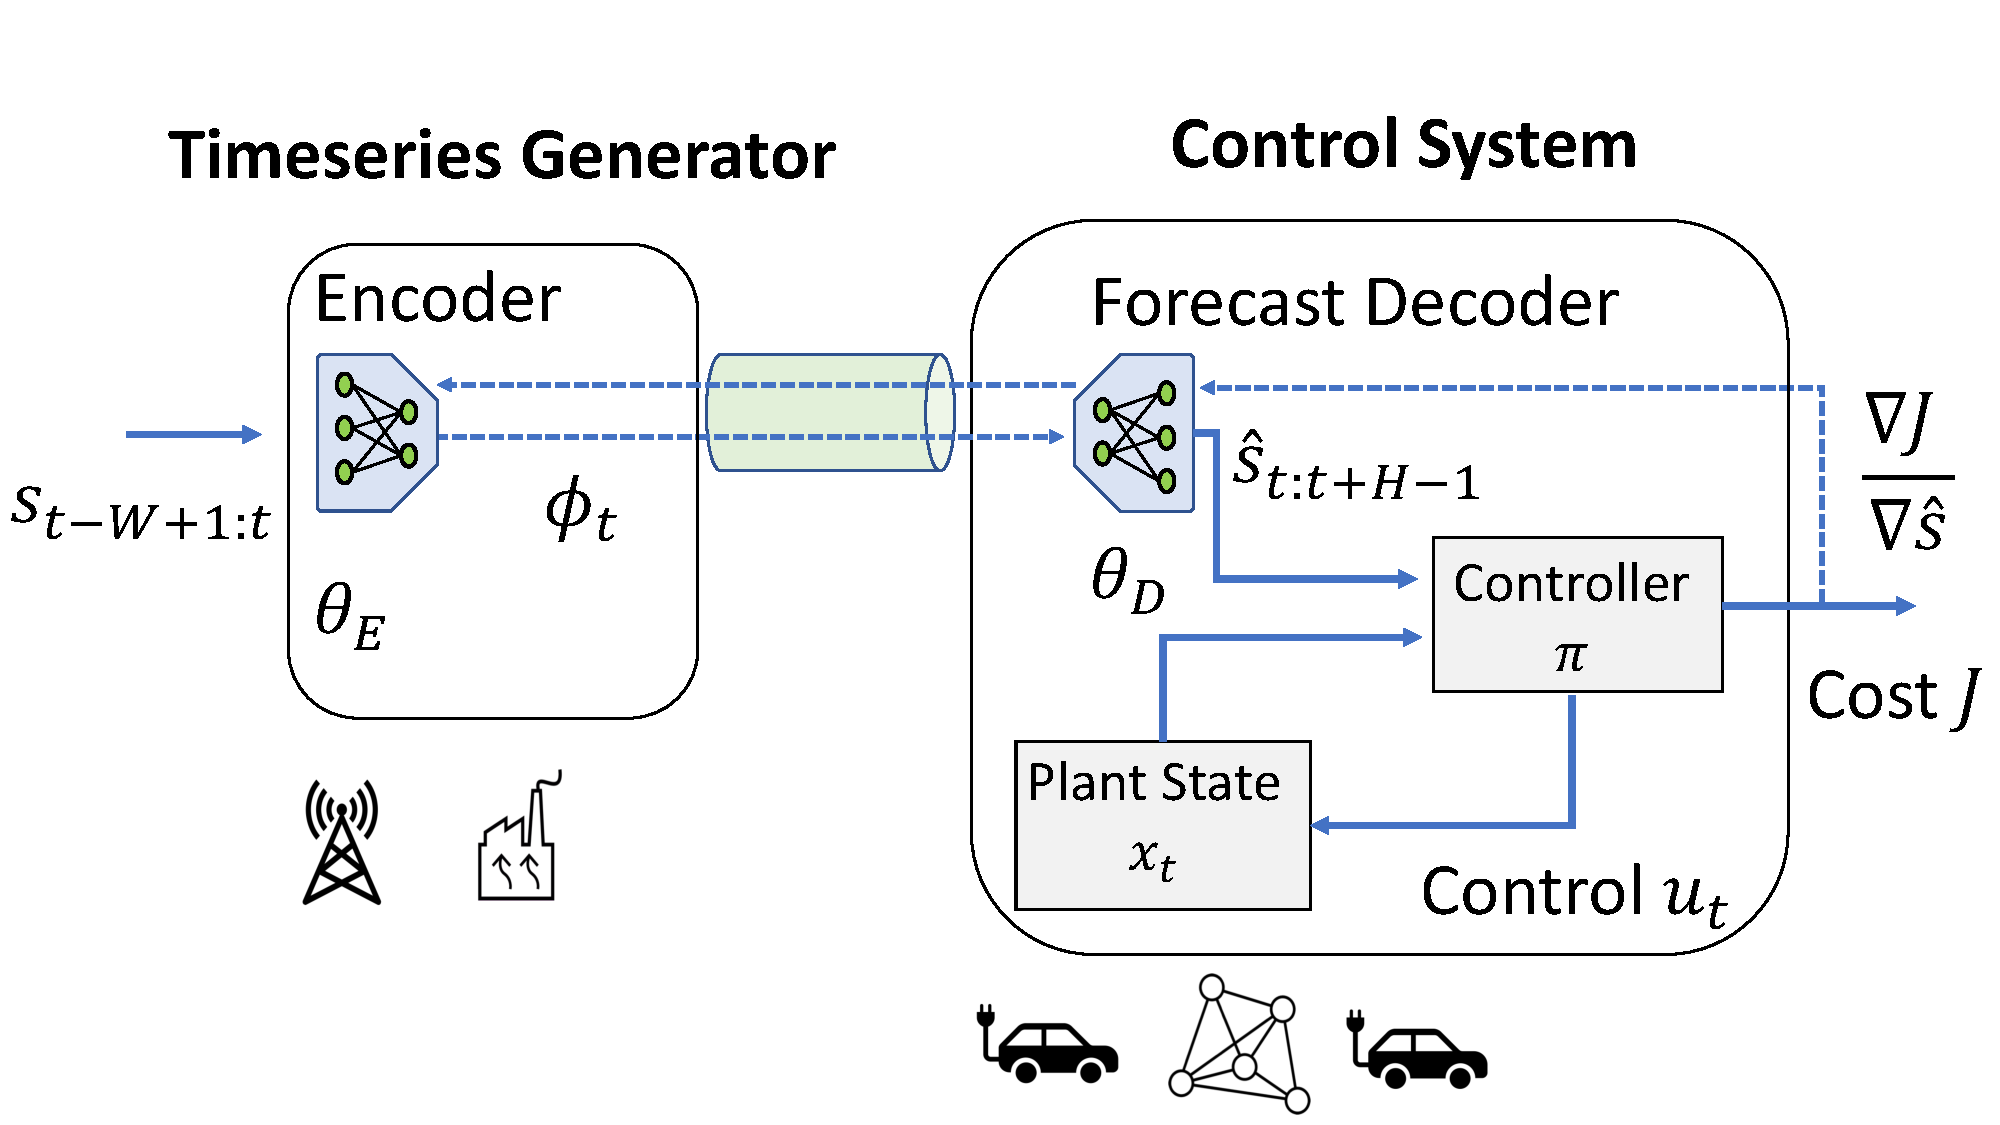
\includegraphics[width=0.99\columnwidth]{pics/final_model_nabla_2.pdf}
\caption{\textbf{Data sharing for cooperative control:} An owner of timeseries data $s_t$, such as a mobile operator, needs to transmit a compressed representation $\phi_t$ to a downstream controller with internal state $x_t$. The \textit{learned} forecast emphasizes task-relevant temporal features to minimize end-to-end controller cost $J$. \newline
    \SC{\textbf{Figure explanation: } This figure describes information flow and a similar figure should be referenced to introduce key notation in your problem formulation (at least for networking or control papers). Use white color and thick black lines as much as possible. Use color with a purpose. For example, all blue modules are learnable in the above figure, while grey modules are model-based. Describe key uses of color in the text or succinctly in the caption.}}
\label{fig_problem}
% \vskip -0.5em
\end{figure}
